工业图像异常检测以产品的正常外观为参照，识别表面缺损、结构变化及纹理偏离。整张图像的外观差异和少量位置的局部异常提供不同的判断依据，因此采用全局支持向量机与正常局部记忆库构成并行检测分支。两个分支共享冻结的卷积特征，分别计算整图分类分数和局部最近邻距离，再通过训练集内的分数校准与加权融合形成统一评分。

图\ref{fig:method}展示的是全局分类与局部记忆融合的图像异常检测框架。共享特征由预训练 Wide ResNet50-2 提取。全局分支将多层池化向量送入核分类器，局部分支将空间描述子与正常记忆库比较。训练阶段利用折外分数确定参数、校准统计量和阈值；预测阶段复用冻结配置，输出图像级正常或异常标签。

\begin{figure*}[t]
  \centering
  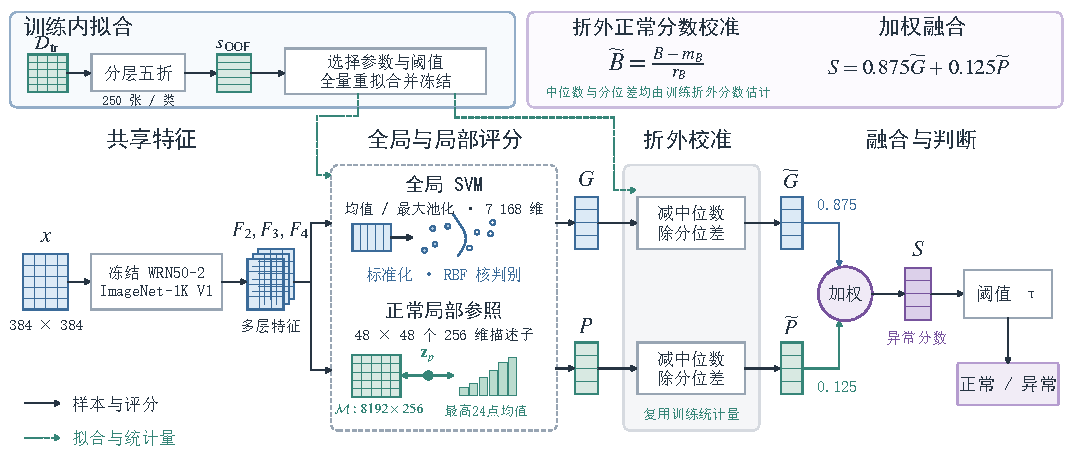
\includegraphics[width=\textwidth]{figures/method-overview.pdf}
  \caption{全局分类与局部记忆融合的工业图像异常检测框架。$m_B,r_B$分别为式\eqref{eq:calibration}中的分数中心与尺度。}
  \Description{共享卷积特征进入全局SVM与局部记忆库两个分支，经折外校准、加权融合与阈值判断得到标签。}
  \label{fig:method}
\end{figure*}

\subsection{任务定义}
设产品类别为$c\in\{\text{榛子},\text{拉链}\}$，其带标签训练集为
\begin{equation}
  \mathcal D_c=\{(\vect x_i,y_i)\}_{i=1}^{N_c},\quad y_i\in\{0,1\},
  \label{eq:data}
\end{equation}
其中$\vect x_i$为RGB图像，$y_i=0$表示正常，$y_i=1$表示异常。学习目标是利用训练图像及其标签构造评分函数$S_c$和阈值$\tau_c$。对已知产品类别的待测图像$\vect x$，判断规则为
\begin{equation}
  \widehat y=\ind\!\left(S_c(\vect x)\geq\tau_c\right).
  \label{eq:decision}
\end{equation}
较大的分数表示更强的异常倾向。两个产品类别分别建立模型和阈值。训练集同时包含正常与异常图像，因此整体方法使用监督信息；其中局部记忆库仅由正常训练图像建立。

\subsection{共享卷积特征与多尺度表示}
图像解码为RGB后，将完整画面双线性缩放至$384\times384$。像素先映射至$[0,1]$，再使用ImageNet通道均值$(0.485,0.456,0.406)$与标准差$(0.229,0.224,0.225)$进行标准化。该过程保留完整的榛壳与拉链布边，训练、验证和测试使用相同变换。

特征提取器采用 Wide ResNet50-2 的 ImageNet-1K V1 权重\cite{wide,torchvision}。固定网络参数，并在评估模式下使用预训练的批归一化统计量。记\texttt{layer2}、\texttt{layer3}和\texttt{layer4}输出为$\tensor F_2,\tensor F_3,\tensor F_4$，其通道数分别为512、1024和2048，空间网格分别为$48\times48$、$24\times24$和$12\times12$。

全局表示汇总各层的空间均值与最大响应。记$\operatorname{GAP}$和$\operatorname{GMP}$为对应池化算子，则
\begin{equation}
\begin{aligned}
 \vect g(\vect x)&=\mathop{\operatorname{Concat}}_{\ell\in\{2,3,4\}}
 \bigl[\operatorname{GAP}(\tensor F_\ell),\operatorname{GMP}(\tensor F_\ell)\bigr],\\
 \vect g(\vect x)&\in\R^{7168}.
\end{aligned}
\label{eq:global}
\end{equation}
其中$7168=2(512+1024+2048)$。均值池化描述整体响应，最大池化保留较突出的位置，二者共同形成整图表示。

局部表示保留空间对应关系。对$\tensor F_2$和$\tensor F_3$施加$3\times3$、步长为1的均值池化，并将后者双线性插值至$48\times48$。记位置$p$处拼接的1536维向量为$\vect v_p$，固定随机投影为
\begin{equation}
 \vect z_p=\vect v_p\vect R,\quad
 R_{ab}\sim\mathcal N(0,1/256),\quad \vect z_p\in\R^{256}.
 \label{eq:projection}
\end{equation}
矩阵$\vect R\in\R^{1536\times256}$使用种子2026生成，所有图像复用同一矩阵。每张图像得到$48^2=2304$个局部描述子。随机投影减小后续距离计算的维度，而空间网格用于回查高响应位置。

每类仅有250张训练图像，冻结预训练网络将拟合集中在分类器与正常参照上，减少从小规模数据学习大量卷积参数的需求。全局池化提供紧凑的整图表示，但可能弱化小面积缺陷；局部网格保留细节，却也会响应正常纹理变化。设置两个分支是为了同时利用这两类证据。

\subsection{全局支持向量机分支}
对当前拟合集的全局特征逐维估计均值$\mu_j$与标准差$\sigma_j$，得到
\begin{equation}
 u_j=\frac{g_j-\mu_j}{\sigma_j},\quad \vect u\in\R^{7168}.
 \label{eq:standard}
\end{equation}
零方差维度的缩放因子取1。验证和测试图像复用拟合阶段的统计量，避免使用待测样本重新估计特征尺度。

使用径向基核支持向量机学习正常与异常之间的边界\cite{svc}。核函数为
\begin{equation}
 K(\vect u_i,\vect u_j)=\exp\bigl(-\gamma\|\vect u_i-\vect u_j\|_2^2\bigr).
 \label{eq:kernel}
\end{equation}
令$t_i=2y_i-1$，带类别权重的软间隔目标为
\begin{equation}
\begin{aligned}
 \min_{\vect w,b,\vect\xi}\quad&\frac12\|\vect w\|_2^2+C\sum_i a_{y_i}\xi_i,\\
 \text{s.t.}\quad&t_i\bigl(\vect w^\top\phi(\vect u_i)+b\bigr)\geq1-\xi_i,\\
 &\xi_i\geq0,
\end{aligned}
\label{eq:svm}
\end{equation}
其中$a_k=n/(2n_k)$，$n_k$是拟合集内类别$k$的样本数。类别权重补偿正常与异常样本的数量差异。由支持向量及其系数得到全局分数
\begin{equation}
 G(\vect x)=\sum_{i\in\mathcal V}\beta_i t_i
 K(\vect u_i,\vect u(\vect x))+b.
 \label{eq:gscore}
\end{equation}
$\mathcal V$为支持向量索引集合。较大的$G$表示更接近训练异常样本一侧。

\subsection{正常局部记忆与最近邻分支}
局部分支利用正常图像的局部表示建立参照。该思路借鉴PatchCore的正常局部特征记忆\cite{roth2022}，具体实现采用随机无放回采样，不使用其贪心核心集选择。对当前拟合集中的正常图像，从全部局部描述子中抽取8192个组成记忆库$\mathcal M_c$。

对待测图像位置$p$，计算其到正常记忆库的最近欧氏距离
\begin{equation}
 d_p(\vect x)=\min_{\vect m\in\mathcal M_c}\|\vect z_p(\vect x)-\vect m\|_2.
 \label{eq:distance}
\end{equation}
将2304个距离从大到小记为$d_{(1)}\geq\cdots\geq d_{(2304)}$，局部分数为最高$k$个距离的均值：
\begin{equation}
 P_q(\vect x)=\frac1k\sum_{r=1}^{k}d_{(r)}(\vect x),\quad
 k=\lceil2304q\rceil.
 \label{eq:local}
\end{equation}
该聚合保留少量位置上的高异常响应，并减轻单个极值的影响。每个记忆库保存$8192\times256$个\texttt{float32}数值，占8 MiB。精确最近邻计算按256个查询描述子分块执行，以限制中间距离矩阵的内存开销。

\subsection{折外校准与加权融合}
两个分支的数值范围不同，融合前使用训练集折外分数校准尺度。每个产品类别采用分层五折，保证一张训练图像的折外分数由未使用该图像拟合的模型给出。各折的特征标准化统计量与正常记忆库仅在当前拟合折建立。

对选定分支$B\in\{G,P\}$，取正常训练图像的折外分数，记其第10、50和90百分位数为$Q_{10}^{B}$、$Q_{50}^{B}$和$Q_{90}^{B}$。定义
\begin{equation}
 \widetilde B(\vect x)=\frac{B(\vect x)-Q_{50}^{B}}
 {\max(Q_{90}^{B}-Q_{10}^{B},10^{-8})}.
 \label{eq:calibration}
\end{equation}
中位数用于对齐正常分数中心，分位数跨度用于统一尺度。校准分数可以小于0或大于1，不解释为异常概率。

给定局部分支权重$\alpha$，融合分数为
\begin{equation}
 S_c(\vect x)=(1-\alpha)\widetilde G(\vect x)+\alpha\widetilde P(\vect x).
 \label{eq:fusion}
\end{equation}
先分别选择全局分支与局部分支的参数，再在选定分支的折外分数上选择$\alpha$。每组候选分数的阈值取相邻不同分数的中点及两端候选，以F1为首要目标；并列时依次比较平衡准确率、召回率，最后取较低阈值。参数候选按F1、平衡准确率和AUROC依次比较。

确定配置后，使用每类全部训练图像重拟合SVM与正常记忆库，并保留折外校准统计量及阈值。测试阶段先保存冻结配置，再计算并保存图像分数和预测，最后与官方标签关联以计算指标。五折结果用于参数选择与校准，不作为独立的泛化性能估计。
